\documentclass[a4paper,12pt]{report}
\usepackage{amsmath}
\usepackage{latexsym}
\usepackage{amsfonts}
\usepackage{amssymb}
\usepackage{graphicx}
\usepackage{txfonts}
\usepackage{wasysym}
\usepackage{wrapfig}
\usepackage{enumitem}
\usepackage{adjustbox}
\usepackage{ragged2e}
\usepackage{tabularx}
\usepackage{changepage}
\usepackage{hhline}
\usepackage{float}
\usepackage{multirow}
\usepackage{makecell}
\usepackage{fancyhdr}
\usepackage[toc,page]{appendix}
\usepackage[utf8]{inputenc}
\usepackage[T1]{fontenc}
\usepackage{hyperref}
\hypersetup{
colorlinks=true,
linkcolor=blue,
filecolor=magenta,
urlcolor=cyan,
}
\urlstyle{same}
\setcounter{tocdepth}{5}
\setcounter{secnumdepth}{5}
\usepackage[a4paper,bindingoffset=0.2in,headsep=0.5cm,left=1in,right=1in,bottom=2cm,top=4cm,headheight=4cm]{geometry}
\everymath{\displaystyle}
\setlistdepth{9}
\newlist{myEnumerate}{enumerate}{9}
	\setlist[myEnumerate,1]{label=\arabic*)}
	\setlist[myEnumerate,2]{label=\alph*)}
	\setlist[myEnumerate,3]{label=(\roman*)}
	\setlist[myEnumerate,4]{label=(\arabic*)}
	\setlist[myEnumerate,5]{label=(\Alph*)}
	\setlist[myEnumerate,6]{label=(\Roman*)}
	\setlist[myEnumerate,7]{label=\arabic*}
	\setlist[myEnumerate,8]{label=\alph*}
	\setlist[myEnumerate,9]{label=\roman*}

\renewlist{itemize}{itemize}{9}
	\setlist[itemize]{label=$\cdot$}
	\setlist[itemize,1]{label=\textbullet}
	\setlist[itemize,2]{label=$\circ$}
	\setlist[itemize,3]{label=$\ast$}
	\setlist[itemize,4]{label=$\dagger$}
	\setlist[itemize,5]{label=$\triangleright$}
	\setlist[itemize,6]{label=$\bigstar$}
	\setlist[itemize,7]{label=$\blacklozenge$}
	\setlist[itemize,8]{label=$\prime$}

\pagestyle{fancy}
\fancyhf{}
\chead{\begin{center}UMANG DESHPANDE\end{center} \\
\begin{center}spdu02@gmail.com  $  \vert  $  +91 7350368207  $  \vert  $  \href{numbering.xml}{www.linkedin.com/in/umang-deshpande}
\end{center} \\
\vspace{12pt}
}
\rfoot{\thepage}
\begin{document}
\sloppy 
\begin{wrapfigure}{r}{1.0in}
\begin{flushright}
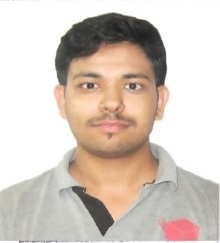
\includegraphics[width=1.0in,height=1.1in]{./image1.jpeg}
\end{flushright}
\end{wrapfigure}
\vspace{12pt}
\noindent E-2,Nirant Society,  \\
Kothari blocks, \\
Near Sahyadri Hospital, \\
Bibwewadi,Pune \\
\vspace{12pt}
\\
\\
\\
\vspace{36pt}
\begin{adjustwidth}{-0.59in}{-0.52in}
\textbf{OVERVIEW} \\
\\
I am a third year undergraduate student in the Electronics and Telecommunication department at the Pune Institute of Computer Technology. My research interest lies in Embedded Systems, Artificial Intelligence and Robotics.
\end{adjustwidth}

\vspace{12pt}
\begin{adjustwidth}{-0.59in}{-0.52in}
\\
\vspace{1cm}
\textbf{EDUCATION}
\end{adjustwidth}
 \\
\vspace{12pt}
\begin{table}[H]
\centering
\begin{adjustbox}{width=\textwidth}
\begin{tabular}{ p{1.08in}p{1.77in}p{3.64in}p{0.89in} }
\hhline{----}
\multicolumn{1}{|p{1.08in}}{Year
} & \multicolumn{1}{|p{1.77in}}{Degree
} & \multicolumn{1}{|p{3.64in}}{Institution (Board)
} & \multicolumn{1}{|p{0.89in}|}{CGPA/%
} & \hhline{----}
\multicolumn{1}{|p{1.08in}}{2014-present
} & \multicolumn{1}{|p{1.77in}}{Bachelor of Engineering
} & \multicolumn{1}{|p{3.64in}}{Pune Institute of Computer Technology (pursuing)
} & \multicolumn{1}{|p{0.89in}|}{72.77%
} & \hhline{----}
\multicolumn{1}{|p{1.08in}}{2014
} & \multicolumn{1}{|p{1.77in}}{XII
} & \multicolumn{1}{|p{3.64in}}{Fergusson College, Pune (H.S.C.)
} & \multicolumn{1}{|p{0.89in}|}{92%
} & \hhline{----}
\multicolumn{1}{|p{1.08in}}{2012
} & \multicolumn{1}{|p{1.77in}}{X
} & \multicolumn{1}{|p{3.64in}}{Kendriya Vidyalaya, Aurangabad (C.B.S.E.)
} & \multicolumn{1}{|p{0.89in}|}{10.0 CGPA
} & \hline
\end{tabular}
\end{adjustbox}
\end{table}


\begin{adjustwidth}{-0.59in}{-0.52in}
\\
\vspace{1cm}
\textbf{RELEVANT COURSES:} 
\end{adjustwidth}
 \\
\begin{adjustwidth}{-0.59in}{0.0in}
\\
Micro Controller Applications and Embedded Processors, Digital Signal Processing, Signals and Systems, Data Structures and Algorithms, Control Systems, Object Oriented Programming, System Programming and operating System, Information Theory and Coding Techniques, Computer Organisation
\end{adjustwidth}
 \\
\vspace{12pt}


\begin{adjustwidth}{-0.59in}{-0.52in}
\\
\vspace{1cm}
\textbf{CERTIFIED COURSES}
\end{adjustwidth}
 \\
\begin{itemize}
\item PCB Designing \hspace*{20pt}  \hspace*{20pt}        \hspace*{20pt}                                                                                            July’16 – Sept’16 \\
\item Roboctics Workshop and training program- Campus Component Pvt. Ltd         \hspace*{20pt}                    Sept’14 \\
\vspace{12pt}
\end{itemize}

\begin{adjustwidth}{-0.59in}{-0.52in}
\\
\vspace{1cm}
\textbf{TECHNICAL KNOWLEDGE}
\\
\textbf{Programming}      \hspace{10pt} C, C++, JAVA, Python, MATLAB, Open CV, Assembly level
 \\
\\
\textbf{Mathematics}       \hspace{10pt} Probability theory, Random Processes, Fourier analysis
 \\
\\
\textbf{Software} \hspace{10pt}      \hspace{10pt} Multisim, Modelsim, MPLAB, Proteus, LabVIEW, AVRStudio, Atmel Studio,  Eagle, \hspace{10pt} SolidWorks
 \\
\\
\textbf{Hardware} \hspace{10pt} PIC18F4550, LPC2148, LPC1768, ATmega2560, Intel8085
\end{adjustwidth}


\begin{adjustwidth}{-0.59in}{0.0in}
\\
\vspace{1cm}
\textbf{PROJECT EXPERIENCE}
\end{adjustwidth}
 \\
\vspace{12pt}
\begin{adjustwidth}{0.0in}{-0.52in}
\\
All Terrain Bot (MINI PROJECT- COLLEGE COURSE)  \hspace{10pt}  \hspace{10pt}  \hspace{10pt}        \hspace{10pt}                                   Dec’16 – April’17
\end{adjustwidth}
 \\
\begin{itemize}
\item Designing a bot capable of walking in all terrain. Inspired from RHex. \\
\end{itemize}
\begin{adjustwidth}{0.0in}{-0.52in}
\\
E-Yantra Ideas Competition – IIT BOMBAY                                                                                                         Jan’17-March’17
\end{adjustwidth}
 \\
\begin{itemize}
\item Designing a bot capable of walking in any terrain, Human detection using Image Processing techniques  for Rescue operations \\
\end{itemize}
\begin{adjustwidth}{0.0in}{-0.52in}
\\
ROBOCON 2017;16;15                                                                                                                                             Aug’14-March’17
\end{adjustwidth}
 \\
\begin{itemize}
\item Designing PCBs, Interfacing of sensors such as sharp, compass, zibee,etc. Power Management. \\
\end{itemize}
\begin{adjustwidth}{0.0in}{-0.52in}
\\
E-Yantra Robotics Competition – IIT BOMBAY \hspace{10pt}  \hspace{10pt}  \hspace{10pt}  \hspace{10pt}  \hspace{10pt}  \hspace{10pt}   \hspace{10pt}    Aug’16 – March’17
\end{adjustwidth}
 \\
\begin{itemize}
\item Applied the concepts of Image processing, wireless communication, path planning algorithms, obstacle and crater avoidance to reach safely to the base station. \\
\vspace{12pt}
\vspace{12pt}
\end{itemize}

\end{document}